\rhead{MODELES DE TURBULENCE}
\chapter{Introduction}
\lhead{Introduction}
\rhead{MODELES DE TURBULENCE}
Les mod\`eles et m\'ethodes num\'eriques de turbulence peuvent \^etre class\'ees
en trois cat\'egories selon les \'echelles r\'esolues : (1) la m\'ethode de
simulation num\'erique directe (Direct Numerical Simulation -- DNS),
(2) la simulation des grandes \'echelles (Large Eddy Simulation -- LES)
et (3) la m\'ethode des \'equations de Navier-Stokes moyenn\'ees (Reynolds-Averaged
Navier-Stokes -- RANS). La DNS r\'esout les \'equations de Navier-Stokes
sans mod\`ele de turbulence et toutes les \'echelles spatiales et temporelles
de la turbulence sont r\'esolues. Par cons\'equent, le maillage en DNS
doit \^etre suffisamment fin pour capturer les tourbillons de tailles
s'\'etendant de la plus petite \'echelle de dissipation (\'echelle de Kolmogorov)
jusqu'\`a l'\'echelle de longueur caract\'eristique de la taille du domaine.
La th\'eorie de la turbulence montre que le nombre de points du maillage
en DNS 3D est de l'ordre de $O(\mbox{Re}^{9/4})$ o\`u $\mbox{Re}$
est le nombre de Reynolds turbulent. Les co\^uts de calcul de la DNS
sont par cons\'equent tr\`es importants pour des forts nombres de Reynolds.

Contrairement \`a la DNS, la LES r\'esout seulement les grandes structures
des \'ecoulements en filtrant les \'equations de Navier-Stokes avec un
filtre spatial et la petite \'echelle non r\'esolue est mod\'elis\'ee en utilisant
des mod\`eles de sous-grille. La gamme des \'echelles r\'esolues en LES
est beaucoup plus petite qu'en DNS et par cons\'equent les co\^uts de
calcul sont r\'eduits de fa\c con significative. On pr\'esentera les deux
principaux mod\`eles LES dans la section \ref{sec:LES}.

Enfin, les mod\`eles RANS sont compos\'es d'un ensemble d'\'equations de
Navier-Stokes moyenn\'ees, avec des mod\`eles de turbulence pour fermer
le tenseur de Reynolds suppl\'ementaire qui est induit par les fluctuations.
Les mod\`eles RANS r\'esolvent seulement l'\'ecoulement moyen aux \'echelles
macroscopiques et il s'agit de la m\'ethode la plus \'economique pour
la simulation de la turbulence. Dans la suite on pr\'esente un des mod\`eles
RANS dans la section \ref{sec:Modele-RANS}.


\chapter{\label{sec:LES}Simulations des grandes \'echelles}
\lhead{Simulations des grandes \'echelles}
\rhead{MODELES DE TURBULENCE}
L'approche de la turbulence bas\'ee sur la Simulation des Grandes Echelles
(SGE, ou Large Eddy Simulation -- LES) consiste \`a obtenir par r\'esolution
directe des \'equations de Navier-Stokes, les caract\'eristiques de grande
taille de la turbulence pour n'avoir \`a mod\'eliser que les mouvements
de \og petite taille \fg{}. Les contributions des grandes \'echelles
sont isol\'ees en introduisant un op\'erateur de moyenne spatiale filtr\'ee
: $\tilde{f}(\mathbf{x},\,t)=\int_{V}G(\mathbf{x},\,\mathbf{x}')f(\mathbf{x}',\,t)dV$
et toute fonction du champ de l'\'ecoulement est d\'ecompos\'ee en $f(\mathbf{x},\,t)=\tilde{f}(\mathbf{x},\,t)+f'(\mathbf{x},\,t)$
o\`u $f'(\mathbf{x},\,t)$ est la fluctuation de sous-maille.

En appliquant l'op\'erateur de moyenne filtr\'ee aux \'equations du mouvement
on obtient :

\begin{subequations}

\begin{eqnarray}
\frac{\partial\tilde{u}_{j}}{\partial x_{j}} & = & 0\label{eq:divu_LES}\\
\frac{\partial\tilde{u}_{i}}{\partial t}+\frac{\partial}{\partial x_{j}}(\widetilde{u_{i}u_{j}}) & = & \frac{1}{\rho_{0}}\frac{\partial\tilde{p}}{\partial x_{i}}+\nu\frac{\partial^{2}\tilde{u}_{i}}{\partial x_{j}\partial x_{j}}\label{eq:QDM_LES}
\end{eqnarray}


\end{subequations}

La moyenne spatiale filtr\'ee du produit $\widetilde{u_{i}u_{j}}$ est
r\'e\'ecrite sous la forme :

\[
\widetilde{u_{i}u_{j}}=\tilde{u}_{i}\tilde{u}_{j}+\tilde{L}_{ij}+\tilde{R}_{ij}
\]
o\`u :

\begin{subequations}

\begin{eqnarray}
\tilde{L}_{ij} & = & \widetilde{\tilde{u}_{i}\tilde{u}_{j}}-\tilde{u}_{i}\tilde{u}_{j}\label{eq:Tension-Leonard}\\
\tilde{R}_{ij} & = & \widetilde{\tilde{u}_{i}u_{j}'}+\widetilde{\tilde{u}_{j}u_{i}'}+\widetilde{u_{i}'u_{j}'}\label{eq:Tension-Reynolds}
\end{eqnarray}


\end{subequations}

La relation (\ref{eq:Tension-Leonard}) caract\'erise les tensions de
Leonard tandis que la relation (\ref{eq:Tension-Reynolds}) caract\'erise
les tensions de Reynolds de sous-maille. Le probl\`eme de fermeture
de la proc\'edure SGE consiste \`a d\'eterminer une relation de $\tilde{R}_{ij}$
pour obtenir la solution d'une r\'ealisation de l'\'ecoulement.


\subsection{Smagorinski}

Le tenseur des contraintes de sous-maille $\tilde{R}_{ij}$ peut \^etre
repris sous la forme :

\[
\tilde{R}_{ij}=\tilde{T}_{ij}+\frac{1}{3}\tilde{R}_{kk}\delta_{ij}
\]


Un des mod\`eles de sous-maille tr\`es r\'epandu est celui de Smagorinsky
qui suppose une relation lin\'eaire du tenseur anisotrope $\tilde{T}_{ij}$
avec le champ des d\'eformations filtr\'e $\tilde{S}_{ij}$ telle que
:

\[
\tilde{T}_{ij}=-2\nu_{T}\tilde{S}_{ij}
\]


La viscosit\'e tourbillonnaire des structures de sous-maille $\nu_{T}$
est choisie telle que :

\begin{equation}
\nu_{T}=(C_{S}\Delta)^{2}\sqrt{\sum_{ij}\tilde{S}_{ij}\tilde{S}_{ij}}\label{eq:nu_T_smago}
\end{equation}
o\`u $\Delta$ est l'\'epaisseur du filtre et $C_{S}$ est une constante
positive qui peut varier selon les applications. Dans \cite[p. 2203]{Weickert_etal_CAMWA2009}
les auteurs disent que la valeur peut varier de $C_{S}=0.05$ \`a $C_{S}=0.16$.
Dans \texttt{TrioCFD} la valeur peut \^etre sp\'ecifi\'ee dans le fichier
de donn\'ees d'entr\'ee. Par d\'efaut, elle est fix\'ee \`a $C_{S}=0.18$ si
elle n'est pas.


\subsection{LES-WALE}

Le mod\`ele alternatif est le mod\`ele LES-WALE (Wall Adaptative Local
Eddy-viscosity) \cite{Nicoud-Ducros_LES-WALE_FTC1999} :

\begin{equation}
\nu_{T}=(C_{W}\Delta)^{2}\frac{(\tilde{S}_{ij}^{d}\tilde{S}_{ij}^{d})^{3/2}}{(\tilde{S}_{ij}\tilde{S}_{ij})^{5/2}+(\tilde{S}_{ij}^{d}\tilde{S}_{ij}^{d})^{5/4}}\label{eq:nu_WALE}
\end{equation}
avec

\[
\tilde{S}_{ij}^{d}=\tilde{S}_{ik}\tilde{S}_{kj}+\tilde{\Omega}_{ik}\tilde{\Omega}_{kj}-\frac{1}{3}\delta_{ij}\left(\tilde{S}_{mn}\tilde{S}_{mn}-\tilde{\Omega}_{mn}\tilde{\Omega}_{mn}\right)
\]
o\`u $\tilde{\Omega}{}_{ij}$ est d\'efini par 

\[
\tilde{\Omega}_{ij}=\frac{1}{2}\left(\frac{\partial\tilde{u}_{i}}{\partial x_{j}}-\frac{\partial\tilde{u}_{j}}{\partial x_{i}}\right)
\]


Dans l'Eq. (\ref{eq:nu_WALE}), $\Delta$ est choisi \`a la taille de
maille. Lorsque la valeur $C_{S}$ est \'egale \`a 0.18, une valeur appropri\'ee
de $C_{w}$ est comprise entre $0.55\leq C_{w}\leq0.6$ \cite[p. 170]{Nicoud-Ducros_LES-WALE_FTC1999}.
Dans certaines conditions d'\'ecoulements d\'ecrites dans \cite[sec 3.1]{Nicoud-Ducros_LES-WALE_FTC1999},
la valeur la plus adapt\'ee est $C_{w}=0.5$, et c'ewst celle choisie
dans les simulations (\cite[pp. 191 and 192]{Nicoud-Ducros_LES-WALE_FTC1999}).


\chapter{\label{sec:Modele-RANS}Mod\`ele RANS}
\lhead{Mod\`ele RANS}
\rhead{MODELES DE TURBULENCE}

\section{\'Equations de Reynolds}

La vitesse $\mathbf{u}(\mathbf{x},\,t)$ et la pression $p(\mathbf{x},\,t)$
du champ d'\'ecoulement d'un fluide incompressible sont r\'egies ind\'ependamment
de la temp\'erature par les \'equations de continuit\'e et de la quantit\'e
de mouvement :

\begin{align}
\boldsymbol{\nabla}\cdot\mathbf{u} & =0,\label{eq:ContinuiteMP-2}\\
\rho_{0}\left[\frac{\partial\mathbf{u}}{\partial t}+\mathbf{u}\cdot\boldsymbol{\nabla}\mathbf{u}\right] & =-\boldsymbol{\nabla}p+\eta_{0}\boldsymbol{\nabla}^{2}\mathbf{u}+\rho_{0}\mathbf{F}_{v}\label{eq:DBF-1-2}
\end{align}


Lorsque la vitesse et la pression sont trait\'ees comme des fonctions
al\'eatoires de l'espace et du temps dont on d\'ecompose les valeurs instantan\'ees
en :

\begin{eqnarray*}
\mathbf{u}(\mathbf{x},\,t) & = & \overline{\mathbf{U}}(\mathbf{x},\,t)+\tilde{\mathbf{u}}(\mathbf{x},\,t)\\
p(\mathbf{x},\,t) & = & \overline{P}(\mathbf{x},\,t)+\tilde{p}(\mathbf{x},\,t)
\end{eqnarray*}
o\`u le symbole $\overline{()}$ indique l'op\'erateur de moyenne statistique
(ou moyenne d'ensemble) et le symbole $\tilde{()}$ les fluctuations
(ou \'ecarts par rapport \`a ces moyennes), les \'equations moyenn\'ees de
masse et de quantit\'e de mouvement se traduisent par \cite[sec 4 p 73--76]{Book_Chassaing}
:

\begin{align}
\boldsymbol{\nabla}\cdot\overline{\mathbf{U}} & =0,\label{eq:ContinuiteMasse_Moyennee}\\
\rho_{0}\left[\frac{\partial\overline{\mathbf{U}}}{\partial t}+\overline{\mathbf{U}}\cdot\boldsymbol{\nabla}\overline{\mathbf{U}}\right] & =\boldsymbol{\nabla}\cdot\overline{\boldsymbol{\Sigma}}+\rho_{0}\overline{\mathbf{F}}_{v}\label{eq:QDM_Moyennee}
\end{align}
avec :

\begin{equation}
\overline{\boldsymbol{\Sigma}}=-\overline{P}\mathbf{I}+2\eta_{0}\overline{\mathbf{S}}-\rho_{0}\overline{\tilde{\mathbf{u}}\tilde{\mathbf{u}}}\qquad\mbox{et}\qquad\overline{\mathbf{S}}=\frac{1}{2}(\boldsymbol{\nabla}\overline{\mathbf{U}}+\boldsymbol{\nabla}^{T}\overline{\mathbf{U}})\label{eq:TenseurReynolds}
\end{equation}


Le bilan de quantit\'e de mouvement moyenne est appel\'ee l'\'equation de
Reynolds. Dans cette \'equation, les forces de surface font appara\^itre
un terme suppl\'ementaire $-\rho_{0}\overline{\tilde{\mathbf{u}}\tilde{\mathbf{u}}}$
qui repr\'esente l'agitation turbulente. Le syst\`eme d'\'equations est
ouvert en raison de la pr\'esence des corr\'elations des vitesses fluctuantes
$\overline{\tilde{\mathbf{u}}\tilde{\mathbf{u}}}$.


\section{Mod\`ele $(\overline{k},\,\overline{\epsilon})$}

De nombreuses mod\'elisations du tenseur de Reynolds sont possibles,
mais nous nous int\'eressons ici \`a la plus classique, bas\'ee sur l\textquoteright hypoth\`ese
de Boussinesq : 

\begin{equation}
\overline{\tilde{\mathbf{u}}\tilde{\mathbf{u}}}=-\nu_{T}2\mathbf{\overline{S}}+\frac{2}{3}\overline{k}\mathbf{I}\label{eq:Hyp_Boussinesq}
\end{equation}
o\`u $\nu_{T}$ est une viscosit\'e turbulente scalaire qui traduit les
effets d\textquoteright agitation turbulente. Le terme en $\overline{k}$
au second membre s\textquoteright apparente \`a une pression par agitation
turbulente et est int\'egr\'e dans la pression $\overline{P}$. On obtient
ainsi une \'equation ferm\'ee pour la vitesse moyenne. Dans le cadre du
mod\`ele \`a deux \'equations $\overline{k}$--$\overline{\epsilon}$ qui
nous int\'eresse, une analyse dimensionnelle donne pour la viscosit\'e
turbulente :

\begin{equation}
\nu_{T}=C'_{\eta}\frac{\overline{k}^{2}}{\overline{\epsilon}}\label{eq:nu_T_RANS}
\end{equation}


Le mod\`ele $\overline{k}$--$\overline{\epsilon}$ permet de fermer
le syst\`eme d'\'equations (\ref{eq:ContinuiteMasse_Moyennee})--(\ref{eq:TenseurReynolds})
en r\'esolvant deux \'equations suppl\'ementaires, une sur l'\'energie cin\'etique
turbulente $\overline{k}$ et l'autre sur le taux de dissipation $\overline{\epsilon}$
suivantes \cite[p. 469]{Book_Chassaing} (repris de \cite[Eq. (2.2-1 et 2.2-2)]{Launder-Spalding_NumCompTurbFlow1974})
:

\begin{subequations}

\begin{eqnarray}
\frac{\partial\overline{k}}{\partial t}+\overline{U}_{j}\frac{\partial\overline{k}}{\partial x_{j}} & = & \nu_{T}\left(\frac{\partial\overline{U}_{i}}{\partial x_{j}}+\frac{\partial\overline{U}_{j}}{\partial x_{i}}\right)\frac{\partial\overline{U}_{i}}{\partial x_{j}}+\frac{\partial}{\partial x_{j}}\left[\frac{\nu_{T}}{\sigma_{k}}\frac{\partial\overline{k}}{\partial x_{j}}\right]-\overline{\epsilon}\label{eq:EnerCinTurb_k}\\
\frac{\partial\overline{\epsilon}}{\partial t}+\overline{U}_{j}\frac{\partial\overline{\epsilon}}{\partial x_{j}} & = & C_{\epsilon_{1}}\nu_{T}\frac{\overline{\epsilon}}{\overline{k}}\left(\frac{\partial\overline{U}_{i}}{\partial x_{j}}+\frac{\partial\overline{U}_{j}}{\partial x_{i}}\right)\frac{\partial\overline{U}_{i}}{\partial x_{j}}+\frac{\partial}{\partial x_{j}}\left[\frac{\nu_{T}}{\sigma_{\epsilon}}\frac{\partial\overline{\epsilon}}{\partial x_{j}}\right]-C_{\epsilon_{2}}\frac{\overline{\epsilon}^{2}}{\overline{k}}\label{eq:TauxDissip_eps}
\end{eqnarray}


\end{subequations}

Les \'equations (\ref{eq:EnerCinTurb_k}) et (\ref{eq:TauxDissip_eps})
sont des \'equations de type advection-diffusion avec des termes source.
Le terme de production d\textquoteright \'energie cin\'etique turbulente
(premier terme du membre de droite) joue un r\^ole important dans les
mod\'elisations pari\'etales. Les valeurs standards des cinq constantes
du mod\`ele $C'_{\eta}$, $C_{\epsilon_{1}}$, $C_{\epsilon_{2}}$,
$\sigma_{k}$ et $\sigma_{\epsilon}$ sont fix\'ees par d\'efaut \`a : $C'_{\eta}=0.09$,
$C_{\epsilon_{1}}=1.44$, $C_{\epsilon_{2}}=1.92$, $\sigma_{k}=1.0$
et $\sigma_{\epsilon}=1.3$. Certaines d'entre elles peuvent aussi
varier selon le type d'\'ecoulement consid\'er\'e (voir table \ref{tab:Synthese-valeurs_Coeffkeps}).

\begin{table}
\begin{centering}
\begin{tabular}{ccccccc}
\hline 
R\'ef\'erence & $C_{\eta}'$ & $\sigma_{k}$ & $\sigma_{\epsilon}$ & $C_{\epsilon_{1}}$ & $C_{\epsilon_{2}}$ & \'ecoulement\tabularnewline
\hline 
\cite{Jones-Launder_IJHMT1972} & 0.09 & 1.0 & 1.3 & 1.55 & 2.00 & Haut Reynolds\tabularnewline
\cite{Launder-Sharma_LettHMT1974} & 0.09 & 1.0 & 1.3 & 1.44 & 1.92 & Tourbillonnant\tabularnewline
\cite{Chien_AIAA1982} & 0.09 & 1.0 & 1.3 & 1.35 & 1.92 & Bas Reynolds\tabularnewline
\cite{Fan_etal_AIAA1993} & 0.09 & 1.0 & 1.3 & 1.39 & 1.80 & Bas Reynolds\tabularnewline
\cite{Morgans-etal_Conf1999} & 0.09 & 1.0 & 1.3 & 1.60 & 1.92 & Jet\tabularnewline
\cite{Bahari-Hejazi_IJPMS2009} & 0.09 & 1.0 & 1.3 & 1.40 & 1.92 & Flottabilit\'e\tabularnewline
\hline 
\end{tabular}
\par\end{centering}

\protect\caption{\label{tab:Synthese-valeurs_Coeffkeps}Synth\`ese des valeurs des param\`etres
du mod\`ele $\overline{k}-\overline{\epsilon}$ (repris de \cite{Genty_RapportCEA_2019}).}
\end{table}

\bigskip

Notonq que, si l'on fait appel au mod\`ele standard k-$\epsilon$, ces deux \'equations sont g\'er\'ees comme une seule \'equation (au format TRUST) avec une inconnue vectorielle (k-$\epsilon$) de dimension 2. On peut \'egalement faire appel au mod\`ele dit \og bic\'ephale \fg, où ces deux \'equations sont consid\'er\'ees s\'epar\'ement, ce qui permet par exemple d'utiliser des conditions aux limites diff\'erentes pour k et $\epsilon$.



\section{Autres mod\`eles \`a deux \'equations}


\subsection*{Mod\`ele $(\overline{k},\,\overline{\epsilon})$-\og r\'ealisable \fg{}}

Alternativement au mod\`ele $(\overline{k},\,\overline{\epsilon})$,
d'autres mod\`eles de fermeture \`a deux \'equations existent dans la litt\'erature
: les mod\`eles $(\overline{k},\,\overline{\epsilon})$ modifi\'es (parmi
eux le $(\overline{k},\,\overline{\epsilon})$-\og r\'ealisable \fg{}
, mod\`ele pour lequel les validations sont en cours). Le mod\`ele $(\overline{k},\,\overline{\epsilon})$-\og r\'ealisable \fg{}
s'\'ecrit \cite[Eq. (22) et (23) p. 233]{Shi_etal_keps-realisable_CF1995}
:

\begin{subequations}

\begin{eqnarray}
\frac{\partial\overline{k}}{\partial t}+\overline{U}_{j}\frac{\partial\overline{k}}{\partial x_{j}} & = & \frac{\partial}{\partial x_{j}}\left(\frac{\nu_{T}}{\sigma_{k}}\frac{\partial\overline{k}}{\partial x_{j}}\right)+\left(2\nu_{T}S_{ij}-\frac{2}{3}\overline{k}\delta_{ij}\right)\frac{\partial\overline{U}_{i}}{\partial x_{j}}-\overline{\epsilon}\label{eq:Eq_k_real}\\
\frac{\partial\overline{\epsilon}}{\partial t}+\overline{U}_{j}\frac{\partial\overline{\epsilon}}{\partial x_{j}} & = & \frac{\partial}{\partial x_{j}}\left[\frac{\nu_{T}}{\sigma_{\epsilon}}\frac{\partial\overline{\epsilon}}{\partial x_{j}}\right]+C_{1}S\epsilon-C_{2}\frac{\overline{\epsilon}^{2}}{\overline{k}+\sqrt{\nu\overline{\epsilon}}}\label{eq:Eq_eps_real}
\end{eqnarray}
avec

\end{subequations}

\begin{subequations}

\begin{equation}
S=\sqrt{2S_{ij}S_{ij}},\quad C_{1}=\max\left\{ 0.43,\,\frac{\eta}{5+\eta}\right\} ,\quad\eta=\frac{S\overline{k}}{\overline{\epsilon}}\label{eq:Coeff1_real}
\end{equation}
et \cite[Eq. (19) p. 232 et (21) p. 233]{Shi_etal_keps-realisable_CF1995}
:

\begin{equation}
C_{\eta}=\frac{1}{A_{0}+A_{s}U^{(*)}\frac{\overline{k}}{\overline{\epsilon}}},\quad\mbox{o\`u }A_{0}=4,\quad A_{s}=\sqrt{6}\cos\phi,\quad\phi=\frac{1}{3}\arccos\left(\sqrt{6}W\right),\quad W=\frac{S_{ij}S_{jk}S_{ki}}{(S_{ij}S_{ij})^{3/2}}\label{eq:Coeff2_real}
\end{equation}
et une vitesse $U^{(*)}$ calcul\'ee par \cite[Eq. (20) p. 232]{Shi_etal_keps-realisable_CF1995}

\begin{equation}
U^{(*)}=\sqrt{S_{ij}S_{ij}+\tilde{\Omega}_{ij}\tilde{\Omega}_{ij}},\quad\tilde{\Omega}_{ij}=\Omega_{ij}-2\epsilon_{ijk}\omega_{k},\quad\Omega_{ij}=\overline{\Omega}_{ij}\epsilon_{ijk}\omega_{k}\label{eq:Coeff3_real}
\end{equation}
o\`u $\overline{\Omega}_{ij}$ est le taux de rotation moyen dans un
rep\`ere de r\'ef\'erence en rotation de vitesse angulaire $\omega_{k}$.

\end{subequations}

Dans \texttt{TrioCFD}, ce mod\`ele $(\overline{k},\,\overline{\epsilon})$-\og r\'ealisable \fg{}
a \'et\'e d\'evelopp\'e et valid\'e dans \cite{Angeli_Leterrier_keps-real_NT2018}.


\section{Mod\`ele \og bas Reynolds \fg{}}

Les lois de paroi, \'etablies \`a partir de r\'esultats exp\'erimentaux, permettent
d\textquoteright \'eviter de calculer la solution des \'equations de Navier-Stokes
et du mod\`ele de turbulence proche de la paroi. Le mod\`ele $(\overline{k},\,\overline{\epsilon})$,
coupl\'e \`a une loi de paroi, permet ainsi de simuler le c\oe ur de
l\textquoteright \'ecoulement en se pr\'eservant d\textquoteright un co\^ut
de calcul trop grand d\^u \`a un maillage trop fin proche de la paroi.
Cependant, ce type de mod\`ele est inadapt\'e lorsque le premier point
du maillage se trouve dans la sous-couche visqueuse ($y^{+}<+30$).
Plus le nombre de Reynolds est haut plus cette sous-couche visqueuse
est d'\'epaisseur n\'egligeable, ce qui rend le mod\`ele $(\overline{k},\,\overline{\epsilon})$
avec loi de paroi bien adapt\'e aux \'ecoulements avec de grand nombre
de Reynolds. C\textquoteright est pourquoi ce mod\`ele est appel\'e \'egalement
mod\`ele $(\overline{k},\,\overline{\epsilon})$ \og haut-Reynolds \fg{}.
Lorsque l\textquoteright on \'etudie des \'ecoulements \`a faible nombre
de Reynolds, la sous-couche visqueuse devient plus importante, ce
qui rend l\textquoteright utilisation d'une loi de paroi inadapt\'ee.
\`a faible nombre de Reynolds, il peut \^etre pr\'ef\'erable d\textquoteright utiliser
des mod\`eles, appel\'es ainsi \og bas-Reynolds \fg{}, qui font d\'esormais
appel \`a des fonctions d\textquoteright amortissement et des termes
d\'ependants de la discr\'etisation pour prendre en compte la r\'esolution
num\'erique de la sous-couche visqueuse. Ces mod\`eles permettent \'egalement
d\textquoteright \'etudier l\textquoteright ensemble de l\textquoteright \'ecoulement
notamment proche de la paroi (par exemple \`a des effets de recirculation,
de d\'ecollement pour des g\'eom\'etries complexes). Le mod\`ele $(\overline{k},\,\overline{\epsilon})$
bas-Reynolds laisse l\textquoteright \'equation de transport de $\overline{k}$
du mod\`ele $(\overline{k},\,\overline{\epsilon})$ de base inchang\'ee
mais modifie celle de $\overline{\epsilon}$ par adjonction de termes
d\textquoteright att\'enuation dans la zone proche de la paroi o\`u le
nombre de Reynolds est localement plus faible. Du fait d\textquoteright un
maillage de paroi important, ce mod\`ele est donc plus co\^uteux que le
mod\`ele $(\overline{k},\,\overline{\epsilon})$ standard. Il existe
plusieurs mod\`eles bas-Reynolds dans la litt\'erature \cite{Launder-Sharma_LettHMT1974,Launder-Spalding_NumCompTurbFlow1974,Jones-Launder_IJHMT1972,Lam-Bremhorst_JFE1981}.
La forme g\'en\'erale de ces mod\`eles peut s'\'ecrire sous la forme (\'ecriture
inspir\'ee de \cite{Jones-Launder_IJHMT1972}) :

\begin{subequations}

\begin{eqnarray}
\frac{\partial\overline{k}}{\partial t}+\overline{U}_{j}\frac{\partial\overline{k}}{\partial x_{j}} & = & \nu_{T}\left(\frac{\partial\overline{U}_{i}}{\partial x_{j}}+\frac{\partial\overline{U}_{j}}{\partial x_{i}}\right)\frac{\partial\overline{U}_{i}}{\partial x_{j}}+\frac{\partial}{\partial x_{j}}\left[\left(\nu+\frac{\nu_{T}}{\sigma_{k}}\right)\frac{\partial\overline{k}}{\partial x_{j}}\right]-\overline{\epsilon}-\overline{\mathcal{K}}\label{eq:EnerCinTurb_k_LowRe}\\
\frac{\partial\overline{\epsilon}}{\partial t}+\overline{U}_{j}\frac{\partial\overline{\epsilon}}{\partial x_{j}} & = & C_{\epsilon_{1}}\nu_{T}\frac{\overline{\epsilon}}{\overline{k}}f_{\epsilon_{1}}\left(\frac{\partial\overline{U}_{i}}{\partial x_{j}}+\frac{\partial\overline{U}_{j}}{\partial x_{i}}\right)\frac{\partial\overline{U}_{i}}{\partial x_{j}}+\frac{\partial}{\partial x_{j}}\left[\left(\nu+\frac{\nu_{T}}{\sigma_{\epsilon}}\right)\frac{\partial\overline{\epsilon}}{\partial x_{j}}\right]-C_{\epsilon_{2}}f_{\epsilon_{2}}\frac{\overline{\epsilon}^{2}}{\overline{k}}+\overline{\mathcal{E}}\label{eq:TauxDissip_eps_LowRe}\\
\nu_{T} & = & C_{\eta}f_{\eta}\frac{\overline{k}^{2}}{\overline{\epsilon}}\label{eq:Nu_T_LowRe}
\end{eqnarray}


\end{subequations}


\subsection*{Mod\`ele \og bas-Reynolds \fg{} de Launder \& Spalding \cite{Launder-Spalding_NumCompTurbFlow1974}}

Pour ce mod\`ele, les termes $\overline{\mathcal{K}}$ et $\overline{\mathcal{E}}$
s'\'ecrivent \cite[Eqs. (2.3-4) et (2.3-5)]{Launder-Spalding_NumCompTurbFlow1974}
:

\begin{equation}
\overline{\mathcal{K}}=2\nu\left(\frac{\partial\overline{k}^{1/2}}{\partial x_{j}}\right)^{2},\quad\overline{\mathcal{E}}=2.0\nu\nu_{T}\left(\frac{\partial^{2}\overline{U}_{i}}{\partial x_{j}\partial x_{l}}\right)\label{eq:K-E_Model1}
\end{equation}
et les fonctions $f_{\epsilon_{1}}$, $f_{\epsilon_{2}}$, $f_{\eta}$
sont donn\'ees par \cite[Eqs. (2.3-6) et (2.3-7)]{Launder-Spalding_NumCompTurbFlow1974}
:

\[
f_{\epsilon_{1}}=1,\quad f_{\epsilon_{2}}=1.0-0.3e^{-Re_{t}^{2}},\quad f_{\eta}=e^{-2.5/(1+Re_{t}/50)}
\]
o\`u $Re_{t}$ est le nombre de Reynolds turbulent d\'efini par $Re_{t}=\overline{k}^{2}/\nu\overline{\epsilon}$.
Les valeurs des coefficients empiriques sont $C_{\eta}=0.09$, $C_{\epsilon_{1}}=1.44$,
$C_{\epsilon_{2}}=1.92$, $\sigma_{k}=1.0$ et $\sigma_{\epsilon}=1.3$.


\subsection*{Mod\`ele de Jones \& Launder \cite{Jones-Launder_IJHMT1972}}

Ce mod\`ele est formul\'e dans la r\'ef\'erence originale \cite{Jones-Launder_IJHMT1972}
en ne consid\'erant qu'une seule d\'eriv\'ee spatiale $\partial/\partial y$
dans les \'equations (\ref{eq:EnerCinTurb_k_LowRe}) et (\ref{eq:TauxDissip_eps_LowRe}).
Dans ce cas, les termes $\overline{\mathcal{K}}$ et $\overline{\mathcal{E}}$
de ce mod\`ele s'\'ecrivent \cite[Eqs. (8) et (9)]{Jones-Launder_IJHMT1972}
:

\[
\overline{\mathcal{K}}=2\nu\left(\frac{\partial\overline{k}^{1/2}}{\partial y}\right)^{2},\quad\overline{\mathcal{E}}=2.0\nu\nu_{T}\left(\frac{\partial^{2}\overline{U}_{i}}{\partial y^{2}}\right)
\]
qui, en 3D s'\'ecrivent de mani\`ere identique aux deux relations de l'\'equation
(\ref{eq:K-E_Model1}). les fonctions $f_{\epsilon_{1}}$, $f_{\epsilon_{2}}$,
$f_{\eta}$ sont donn\'ees par \cite[Eq. (12)]{Jones-Launder_IJHMT1972}
:

\[
f_{\epsilon_{1}}=1,\quad f_{\epsilon_{2}}=1.0-0.3e^{-Re_{t}^{2}},\quad f_{\eta}=e^{-2.5/(1+Re_{t}/50)}
\]


Les param\`etres empiriques du mod\`ele sont donn\'es par \cite[Table 1]{Jones-Launder_IJHMT1972}
: $C_{\eta}=0.09$, $C_{\epsilon_{1}}=1.55$, $C_{\epsilon_{2}}=2$,
$\sigma_{k}=1.0$ et $\sigma_{\epsilon}=1.3$. Ce mod\`ele ne se diff\'erencie
du pr\'ec\'edent (celui de Launder \& Spalding) que par les valeurs des
param\`etres $C_{\epsilon_{1}}$et $C_{\epsilon_{2}}$.


\subsection*{Mod\`ele de Lam \& Bremhorst \cite{Lam-Bremhorst_JFE1981}}

Dans ce mod\`ele les termes $\overline{\mathcal{K}}$ et $\overline{\mathcal{E}}$
dans les \'equations (\ref{eq:EnerCinTurb_k_LowRe}) et (\ref{eq:TauxDissip_eps_LowRe})
sont nuls et les fonctions $f_{\epsilon_{1}}$, $f_{\epsilon_{2}}$,
$f_{\eta}$ sont donn\'ees par \cite[Eq. (11), (12) et (13)]{Lam-Bremhorst_JFE1981}
:

\[
f_{\epsilon_{1}}=1+\left(\frac{A_{c}}{f_{\eta}}\right)^{3},\quad f_{\epsilon_{2}}=1-e^{-Re_{t}^{2}},\quad f_{\eta}=(1-e^{-A_{\eta}Re_{y}})^{2}\left(1+\frac{A_{t}}{Re_{t}}\right)
\]
o\`u $Re_{y}$ est le nombre de Reynolds turbulent qui varie avec la
distance $y$ \`a la paroi et qui est d\'efini par $Re_{y}=\overline{k}^{1/2}y/\nu$.
Les coefficients $A_{\eta}$, $A_{t}$ et $A_{c}$ sont cal\'es en comparant
les r\'esultats num\'eriques \`a des mesures exp\'erimentales. Les valeurs
obtenues sont (\cite[sec. 3.1]{Lam-Bremhorst_JFE1981}) $A_{\eta}=0.0165$,
$A_{t}=20.5$, et $A_{c}=0.05$. Les valeurs des autres coefficients
sont $C_{\epsilon_{1}}=1.44$ et $C_{\epsilon_{2}}=1.92$.


\subsection*{Mod\`ele de Launder \& Sharma \cite{Launder-Sharma_LettHMT1974}}

Ce mod\`ele est formul\'ee pour les \'ecoulements tourbillonnants (disque
en rotation) pour lesquels les coordonn\'ees ind\'ependantes sont $r$
et $y$ o\`u $r$ est la distance radiale \`a l'axe du disque et $y$
est la distance normale \`a la surface du disque. Dans ce cas, des termes
suppl\'ementaires qui impliquent le gradient de $V_{\theta}/r$ apparaissent
dans les \'equations de $\overline{k}$ et de $\overline{\epsilon}$.
Les fonctions $f_{\epsilon_{2}}$ et $f_{\eta}$ et les constantes
sont l\'eg\`erement diff\'erentes \cite[Eqs. (5), (6)]{Launder-Sharma_LettHMT1974}
:

\[
f_{\epsilon_{2}}=1.0-0.3e^{-Re_{t}^{2}},\quad f_{\eta}=e^{-3.4/(1+Re_{t}/50)^{2}}
\]
et \cite[Eqs. (5), (6) et valeurs au-dessous]{Launder-Sharma_LettHMT1974}
$C_{\eta}=0.09$, $C_{\epsilon_{1}}=1.44$, $C_{\epsilon_{2}}=1.92$,
$\sigma_{k}=1.0$ et $\sigma_{\epsilon}=1.3$.


\subsection*{Dans \texttt{TrioCFD}}

Dans \texttt{TrioCFD}, les mod\`eles de turbulence en $(\overline{k},\,\overline{\epsilon})$
\og bas Reynolds \fg{} de Jones \& Launder \cite{Jones-Launder_IJHMT1972}
et celui de Lam \& Bremhorst \cite{Lam-Bremhorst_JFE1981} ont \'et\'e
mis en \oe uvre dans \cite{Peybernes_LowReynolds_NT2016}. Les fonctions
et param\`etres de Launder \& Sharma \cite{Launder-Sharma_LettHMT1974}
sont \'egalement disponibles.


\chapter{Lois de parois}
\lhead{Lois de parois}
\rhead{MODELES DE TURBULENCE}
Dans le cadre des \'etudes de turbulence, en particulier pour des cas
avec des g\'eom\'etries complexes, la r\'esolution des ph\'enom\`enes physiques
ayant lieu en proche paroi est g\'en\'eralement co\^uteuse en terme de temps
de calcul car elle demande un maillage tr\`es fin dans ces zones o\`u
les gradients de vitesse et de temp\'erature sont tr\`es \'elev\'es. Or il
est primordial de pr\'edire correctement ces ph\'enom\`enes car par simple
conservation du d\'ebit, une mauvaise description pari\'etale de la vitesse
entrainera une mauvaise description au c\oe ur de l\textquoteright \'ecoulement.
Plut\^ot que de faire porter l\textquoteright effort sur une r\'esolution
fine, il est alors classique de faire porter l\textquoteright effort
sur une mod\'elisation du gradient de vitesse pari\'etal, qui permet de
conserver un maillage relativement grossier \`a la paroi. Ces approches
sont connues sous le nom de " lois de paroi " ou " traitement de paroi
" (on rencontre tr\`es souvent les termes anglais de " wall functions
" et " wall treatment ") et permettent une diminution notable des
temps de simulation. Elles sont depuis longtemps int\'egr\'ees \`a la plupart
des codes de calcul industriels.

Les lois disponibles avec le mod\`ele $\overline{k}$--$\overline{\epsilon}$
dans \texttt{TrioCFD} sont formul\'ees de mani\`ere \`a d\'ecrire contin\^ument
toute la couche limite. Pour la vitesse adimensionn\'ee, la loi de paroi
de Reichardt est utilis\'ee \cite{Reichardt1940} :

\[
U^{+}=\frac{1}{\kappa}\ln(1+\kappa y^{+})+A\left(1-e^{-y^{+}/11}-\frac{y^{+}}{11}e^{-y^{+}/3}\right)
\]
avec

\[
A=\frac{1}{\kappa}\ln\left(\frac{E}{\kappa}\right)
\]


Les valeurs des constantes sont $\kappa=0.415$ et $E=9.11$. Asymptotiquement,
on retrouve le comportement lin\'eaire lorsque $y^{+}$ tend vers z\'ero,
et le comportement logarithmique lorsque $y^{+}$ devient " grand
". De plus, cette loi donne une description raisonnable de la zone
tampon. Les quantit\'es $\overline{k}$ et $\overline{\epsilon}$ sont
d\'ecrites, pour tout $y^{+}$, par :

\begin{eqnarray*}
\overline{k}^{+} & = & 0.07y^{+2}e^{-y^{+}/9}+\frac{1}{\sqrt{C_{\eta}}}\left(1-e^{-y^{+}/20}\right)^{2}\\
\overline{\epsilon}^{+} & = & \frac{1}{\kappa(y^{+4}+15^{4})^{1/4}}
\end{eqnarray*}


Ces formulations respectent le comportement g\'en\'eralement admis \`a la
paroi, \`a savoir :

\[
\overline{k}(y=0)=0\,;\qquad\frac{d\overline{k}}{dy}(y=0)=0\,;\qquad\frac{d\overline{\epsilon}}{dy}(y=0)=0
\]



\section{Autres mod\`eles de turbulence dans \texttt{TrioCFD}}

Signalons que la loi d\'evelopp\'ee par Ciofalo et Collins \cite{Ciofalo-Collins_NHTB1989}
est \'egalement disponible mais uniquement pour la discr\'etisation VDF
de \texttt{TrioCFD} (maillages cart\'esiens). Il est \'egalement possible
de modifier la valeur des constantes de la loi logarithmique, ou d\textquoteright imposer
la vitesse de frottement, mais cela semble assez peu utile dans les
\'etudes industrielles. Concernant la LES, la loi de Werner et Wengle
est \'egalement impl\'ement\'ee \cite{Werner-Wengle_Proc1991} ainsi que
l\textquoteright approche TBLE (Thin Boundary Layer Equation).


\subsubsection*{Mod\`ele $(\overline{k},\,\overline{\omega})$ \`a venir}

D'autres mod\`eles de type $(\overline{k},\,\overline{\omega})$ existent
dans la litt\'erature tels que les mod\`eles $(\overline{k},\,\overline{\omega})$
et $(\overline{k},\,\overline{\epsilon})$-SST (Shear Stress Transport).
Les syst\`emes d'\'equations de ces mod\`eles sont pr\'esent\'es dans la r\'ef\'erence
\cite[sec 2.3.6 pp. 701--705]{Argyropoulos-Markatos_ReviewTurbulence_AMM2015}
de laquelle on reprend le mod\`ele $(\overline{k},\,\omega)$ pour lequel
la viscosit\'e turbulence est :

\[
\nu_{T}=\frac{\overline{k}}{\tilde{\omega}},\qquad\tilde{\omega}=\max\left\{ \omega,\,C_{lim}\sqrt{\frac{2S_{ij}S_{ij}}{\beta^{*}}}\right\} ,\qquad\mbox{avec }C_{lim}=\frac{7}{8}
\]


Le mod\`ele s'\'ecrit \cite[p. 702]{Argyropoulos-Markatos_ReviewTurbulence_AMM2015}
(repris de \cite{Wilcox_AIAA1988}) :

\begin{eqnarray*}
\frac{\partial\overline{k}}{\partial t}+\overline{U}_{j}\frac{\partial\overline{k}}{\partial x_{j}} & = & \frac{\partial}{\partial x_{j}}\left[\left(\nu+\sigma^{*}\frac{\overline{k}}{\omega}\right)\frac{\partial\overline{k}}{\partial x_{j}}\right]-\beta^{*}\overline{k}\omega+\tau_{ij}\frac{\partial\overline{U}_{i}}{\partial x_{j}}\\
\frac{\partial\omega}{\partial t}+\overline{U}_{j}\frac{\partial\omega}{\partial x_{j}} & = & \frac{\partial}{\partial x_{j}}\left[\left(\nu+\sigma\frac{\overline{k}}{\omega}\right)\frac{\partial\omega}{\partial x_{j}}\right]-\beta\omega^{2}+\frac{\sigma_{d}}{\omega}\frac{\partial\overline{k}}{\partial x_{j}}\frac{\partial\omega}{\partial x_{j}}+a\frac{\omega}{\overline{k}}\tau_{ij}\frac{\partial\overline{U}_{i}}{\partial x_{j}}
\end{eqnarray*}
avec :

\[
\sigma_{d}=\begin{cases}
0 & \mbox{si }\frac{\partial\overline{k}}{\partial x_{j}}\frac{\partial\omega}{\partial x_{j}}\leq0\\
\sigma_{d0} & \mbox{si }\frac{\partial\overline{k}}{\partial x_{j}}\frac{\partial\omega}{\partial x_{j}}>0
\end{cases},\qquad f_{\beta}=\frac{1+85\chi_{\omega}}{1+100\chi_{\omega}},\qquad\chi_{\omega}=\left|\frac{\Omega_{ij}\Omega_{jk}S_{ki}}{(\beta^{*}\omega)^{3}}\right|,\qquad\Omega_{ij}=\frac{1}{2}\left(\frac{\partial\overline{U}_{i}}{\partial x_{j}}-\frac{\partial\overline{U}_{j}}{\partial x_{i}}\right)
\]


Les coefficients sont les suivants :

\[
a=0.52,\quad\beta=\beta_{0}f_{\beta},\quad\beta_{0}=0.0708,\quad\beta^{*}=0.09,\quad\sigma=0.5,\quad\sigma^{*}=0.6,\quad\sigma_{d0}=0.125
\]



\chapter{LES models with Algo\_QC in \texttt{TrioCFD}}
\lhead{Quasi compressible highly anisothermal turbulence}
\section{Solved equations}
The Algo\_QC module in \texttt{TrioCFD} implementes the low mach number equations in the context of quasi compressible equations, aswell as many Thermal-Large Eddy Simulation (T-LES) models.  This approximation aims to narrow the gap between incompressible and compressible Navier-Stokes equations and is suitable for the computation of convection in a fluid in the presence of large density gradients \cite{paolucci_filtering_1982}. The low Mach number equations consider internal wave propagation, but they do not take into account acoustic waves. Thus, the numerical methods developed for incompressible flow can be used. This approximation conducts to divide the pressure into two terms: the thermodynamical pressure which is homogeneous and the mechanical pressure. The Stokes hypothesis is assumed to be true \cite{Papalexandris2019}. The solved equations are the following:



\begin{itemize}
    \item Mass conservation equation
        \begin{equation}
            \frac{\partial \rho}{\partial t} + \frac{\partial \rho U_j}{\partial x_j} = 0
            \label{eq:mass_conserv}
        \end{equation}
    
    \item Momentum conversation equation
    \begin{equation}
        \frac{
            \partial \rho U_i
        }{
            \partial t
        } = - \frac{
            \partial \rho U_j U_i
        }{
            \partial x_j
        } - \frac{\partial P}{\partial x_i} + \frac{\partial \Sigma_{ij}(U, T)}{\partial x_j}
        \label{eq:moment_conserv}
    \end{equation}
    
    \item Energy conservation equation
    \begin{equation}
        \frac{
            \partial
        }{
            \partial x_j
        } U_j = - \frac{1}{\gamma P_0} \Big[  (\gamma -1) \Big( \frac{\partial Q_j }{\partial x_j} \Big) + \frac{\diff P_0}{\diff t}\Big]
        \label{eq:ener_conserv}
    \end{equation}
    
    \item Ideal gas law
    \begin{equation}
        T = \frac{P_0}{\rho r}
        \label{eq:ideal_gas}
    \end{equation}
    With $\rho$ density, $T$ temperature, $\gamma$ the heat capacity, $r=287 \ \text{J} \cdot \text{kg}^{-1} \cdot \text{K}^{-1}$
\end{itemize}

with $t$ the time, $P$ the mechanical pressure, $P_0$ thermo dynamical pressure, $U_i$ the $i^{\text{th}}$ component of velocity, and $x_i$ the Cartesian coordinate in the $i^{\text{th}}$ direction. The Einstein summation convention is employed. The thermodynamical pressure is obtained by integrating Equation~\ref{eq:ener_conserv} over the volume of the studied geometry:

\begin{equation}
    \difffrac{P_0}{t} = -(\gamma -1) \Big( \frac{1}{V} \int Q_j({T}) \diff S_j \Big)
\end{equation}
With V the volume of the computational domain and $S_j$ the boundaries of the investigated domain.

The shear-stress tensor and the conductive heat flux are respectively computed with the functions $\Sigma_{ij}({U}, {T})$ and $Q_j({T})$, assuming Newtonian fluid and Fourier's law, leading to the following expressions:

\begin{equation}
    \Sigma_{ij}({U}, {T}) = \mu ({T}) \Big( \pfrac{{U_i}}{x_j} + \pfrac{{U_j}}{x_i}\Big) - \frac{2}{3}\mu({T}) \pfrac{{U_k}}{x_k} \delta_{ij}
\end{equation}

\begin{equation}
    Q_j({T}) = - \lambda({T})\pfrac{{T}}{x_j}
\end{equation}

where $\mu(T)$ is the dynamic viscosity, $\lambda(T)$ is the thermal conductivity, and $\delta_{ij}$ the Kronecker symbol.
The fluid passing through the channel is air. Sutherland's law \cite{sutherland_viscosity_1893} is used to compute viscosity from temperature:

\begin{equation}
    \mu(T) = \mu_0 \frac{T}{T_0}^{3/2} \frac{T_0 + S}{T + S}
\end{equation}

where $\mu_0 = 1.716 \times 10^{-5} \ \text{Pa}\cdot\text{s}$, $S = 110.4 \ \text{K}$, and $T_0 = 273.15 \ \text{K}$. The Prandtl number is assumed to be constant in this simulation, and the heat capacity at constant pressure $C_p$ is obtained with the average of wall temperatures. The conductivity is deduced from the Prandtl number, the heat capacity at constant pressure, and the viscosity.

\begin{equation}
    \lambda(T) = \frac{C_p}{P_r} \mu(T)
\end{equation}

\begin{figure}
  \begin{center}
    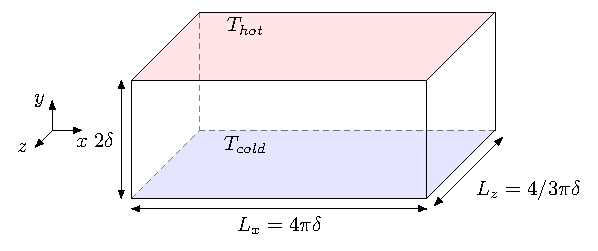
\includegraphics[width=0.95\textwidth]{./figures/canal_plan.pdf}
  \end{center}
  \caption{}
  \label{figure:canal_plan_anisotherme}
\end{figure}


We suppose two boundary temperatures $T_{\text{hot}}$ and $T_{\text{cold}}$, where the temperature differense is of the order of $300K$ to $400K$, with figure~\ref{figure:canal_plan_anisotherme} as a representation.
The streamwise ($x$) and spanwise directions ($z$) are periodic.

A hyperbolic tangent mesh is used in the wall-normal direction ($y$).

The wall-normal grid coordinates are symmetrical with respect to the plane $y=h$. In the first half of the channel, they are given by
\begin{equation}
y_k = h \left( 1 + \frac{1}{a} \tanh\left[ \left(\frac{k-1}{N_y-1} - 1\right)\tanh^{-1}(a)\right] \right), \label{eqmesh}
\end{equation}

with $a$ the mesh dilatation parameter.

\section{Filtered low Mach number equations}\label{label-pa}

We consider the large-eddy simulation of the
low Mach number equations in two formulations as introduced in \cite{dupuy2018study}. The Velocity formulation
expresses the filtered low Mach number equations in terms of variables
filtered with the unweighted classical filter ($\overline{\,\,\cdot\,\,}$).
The Favre formulation expresses the filtered low Mach number equations using
Favre-filtered variables,
that is based on the density-weighted Favre filter ($\fa{\,\,\,\cdot\,\,}$)
defined for any field~$\psi$ as $\fa{\psi} = \f{\rho \psi} / \f{\rho}$.
The two formulations involve a different set of subgrid terms.
However, the two most significant subgrid terms are similar in the two
formulations \cite{dupuy2016, dupuy2017sft, dupuy2018study}.
In both cases, a subgrid term is related to the nonlinearity of momentum
convection and another related to the correlation of density and velocity.
Excluding all other subgrid terms, the filtered low Mach number equations are
given in the Velocity formulation by:
\begin{itemize}
\item Mass conservation equation
\begin{equation}
\der{\f{\rho}}{t} + \der{}{x_j}\left(\f{\rho} \f{U}_{\!j} + F_{\rho U_j}\right) = 0,
\end{equation}
\item Velocity transport equation
\begin{equation}
\begin{aligned}
\der{\f{U}_{\!i}}{t} = - \der{\left(\smash[t]{\f{U}_{\!j} \f{U}_{\!i} + F_{U_j U_i}}\right)}{x_j} + \f{U}_{\!i} \der{\f{U}_{\!j}}{x_j} - \frac{1}{\f{\rho}}\der{\f{P}}{x_i} + \frac{1}{\f{\rho}} \der{\varSigma_{ij}(\vv{\f{U}}, \f{T})}{x_j},
\end{aligned}
\end{equation}
\item Energy conservation equation
\begin{equation}
\der{\f{U}_{\!j}}{x_j} = - \frac{1}{\gamma P_{0}}\left[ (\gamma - 1)\der{Q_j(\f{T})}{x_j} + \der{P_{0}}{t} \right],
\end{equation}
\item Ideal gas law
\begin{equation}
\f{T} = \frac{P_{0}}{r \f{\rho}},
\end{equation}
\end{itemize}
and in the Favre formulation by:
\begin{itemize}
\item Mass conservation equation
\begin{equation}
\der{\f{\rho}}{t} + \der{\f{\rho} \fa{U_{j}}}{x_j} = 0,
\end{equation}
\item Momentum conservation equation
\begin{equation}
\begin{aligned}
\der{\f{\rho} \fa{U}_{\!i}}{t} = - \der{\left(\smash[t]{\f{\rho} \fa{U}_{\!j} \fa{U}_{\!i} + \f{\rho} G_{U_j U_i}}\right)}{x_j} - \der{\f{P}}{x_i} + \der{\varSigma_{ij}(\vv{\fa{U}},\fa{T})}{x_j},
\end{aligned}
\end{equation}
\item Energy conservation equation
\begin{equation}
\der{}{x_j}\left(\fa{U}_{\!j} + \f{\rho} G_{U_j/\rho}\right) = - \frac{1}{\gamma P_{0}}\left[ (\gamma - 1)\der{Q_j(\fa{T})}{x_j} + \der{P_{0}}{t} \right],
\end{equation}
\item Ideal gas law
\begin{equation}
\fa{T} = \frac{P_{0}}{\f{\rho} r},
\end{equation}
\end{itemize}
with $\rho$ the density, $T$ the temperature, $\gamma$ the heat capacity ratio,
$r$ the ideal gas specific constant, $t$ the time, $P$ the mechanical pressure,
$P_0$ the thermodynamical pressure, $U_i$ the $i$-th component of velocity and
$x_i$ the Cartesian coordinate in $i$-th direction. Einstein summation
convention is used.
The functions $\varSigma_{ij}(\vv{U}, T)$ and $Q_j(T)$ are used to compute the
shear-stress tensor and conductive heat flux associated with a given velocity
and temperature. We assume a Newtonian fluid
and Fourier's law,
\begin{align}
\varSigma_{ij}(\vv{U}, T) ={}& \mu(T) \left(\der{U_i}{x_j} + \der{U_j}{x_i}\right) - \frac{2}{3} \mu(T) \der{U_k}{x_k} \delta_{ij}, \\
Q_j(T) {}&= - \lambda(T) \der{T}{x_j},
\end{align}
with $\mu(T)$ the dynamic viscosity, $\lambda(T)$ the thermal conductivity and
$\delta_{ij}$ the Kronecker delta.

The momentum convection subgrid term is defined as
$\smash[t]{F_{U_j U_i} ={} \f{U_j U_i} - \f{U}_{\!j} \f{U}_{\!i}}$ in the Velocity formulation and
$\smash[t]{G_{U_j U_i} ={} \fa{U_j U_i} - \fa{U}_{\!j} \fa{U}_{\!i}}$ in the Favre formulation.
The density-velocity correlation subgrid term is defined as
$\smash[t]{F_{\rho U_j} ={} \f{\rho U_j} - \f{\rho} \f{U}_{\!j}}$ in the Velocity formulation and
$\smash[t]{G_{U_j/\rho} ={} \fa{U_j/\rho} - \fa{U}_{\!j}/\f{\rho}}$ in the Favre formulation.
The two formulations are related by the relation
\begin{equation}
\frac{F_{\rho U_j}}{\f{\rho}} = - \f{\rho} G_{U_j/\rho}.
\end{equation}



The fluid is air. We use Sutherland's law \cite{sutherland1893lii} to compute the viscosity,
\begin{equation}
\mu(T) = \mu_0 \left(\frac{T}{T_0}\right)^{\frac{3}{2}} \frac{T_0 + S}{T + S},
\end{equation}
with $\mu_0 = 1.716\cdot 10^{-5}$~Pa~s, $S=110.4$~K and $T_0 = 273.15$~K.
We assume a constant Prandtl number $Pr = 0.76$ and heat capacity at
constant pressure $C_p~=~1005$~J~kg$^{-1}$~K$^{-1}$.
The conductivity is deduced from the Prandlt number, the heat capacity at
constant pressure and the viscosity,
\begin{equation}
\lambda(T) = \frac{C_p}{Pr} \mu(T).
\end{equation}
The ideal gas specific constant is~$r=287$~J~kg$^{-1}$~K$^{-1}$.


These equations can be solved through the keywork \texttt{large\_eddy\_simulation\_formulation}, with either the \texttt{favre} or \texttt{velocity} values.

the following section is directly taken from~\cite{dupuy2016,dupuy2017sft,dupuy2018study}.

\section{Subgrid-scale models}

The subgrid terms of the Velocity and Favre formulations are formally
similar. Accordingly, the same modelling procedure is used in both cases.
To formalise this, we may express the subgrid-scale models as a function
of the filter length scales and of the filtered velocity and density
in the two formulations:
\begin{align}
F_{U_j U_i} \approx{}& \tau_{ij}^{\mathrm{mod}}(\vv{\f{U}}, \vv{\f{\Delta}}), \\
G_{U_j U_i} \approx{}& \tau_{ij}^{\mathrm{mod}}(\vv{\fa{U}}, \vv{\f{\Delta}}), \\
F_{\rho U_j} \approx{}& \pi_{j}^{\mathrm{mod}}(\vv{\f{U}}, \f{\rho}, \vv{\f{\Delta}}), \\
G_{U_j/\rho} \approx{}& \pi_{j}^{\mathrm{mod}}(\vv{\fa{U}}, 1/\f{\rho}, \vv{\f{\Delta}}),
\end{align}%
where the functions $\tau_{ij}^{\mathrm{mod}}(\vv{U},\vv{\f{\Delta}})$ and
$\pi_j^{\mathrm{mod}}(\vv{U},\phi,\vv{\f{\Delta}})$ are model-dependent but do not depend on the formulation.

Eddy-viscosity models for the subgrid term associated with momentum convection
may be written in the form
\begin{align}
\tau_{ij}^{\mathrm{mod}}(\vv{U}, \vv{\f{\Delta}}) ={}& - 2 \nu_e^{\mathrm{mod}}(\vv{g}, \vv{\f{\Delta}}) S_{ij}, \label{hela}
\end{align}%
with
$S_{ij} = \tfrac{1}{2}\left( g_{ij} + g_{ji} \right)$ the rate of deformation tensor
and
$\vv{g}$
the velocity gradient, defined by $g_{ij} = \partial_j U_i$.
Notice that $\tau_{ij}^{\mathrm{mod}}(\vv{U}, \vv{\f{\Delta}})$ may be
considered traceless without loss of generality, even in the incompressible case,
since the trace can be included as part of the filtered pressure $\f{P}$.
The eddy-viscosity $\nu_e^{\mathrm{mod}}(\vv{g}, \vv{\f{\Delta}})$
is given by the model used.
The following models from the literature are investigated in this paper using a priori tests:
\begin{flalign}
&\textrm{Smagorinsky model \cite{smagorinsky1963general}:} & \nu_e^{\mathrm{Smag.}}  (\vv{g}, \vv{\f{\Delta}}) ={}& \left( C^{\mathrm{Smag.}} \f{\Delta} \right)^2 \left|\vt{S}\right|, &&& \label{sma} \\
&\textrm{WALE model \cite{nicoud99b}:}                     & \nu_e^{\mathrm{WALE}}   (\vv{g}, \vv{\f{\Delta}}) ={}& \left( C^{\mathrm{WALE}} \f{\Delta} \right)^2 \frac{\left(\mathcal{S}^d_{ij} \mathcal{S}^d_{ij}\right)^{\tfrac{3}{2}}}{\left(S_{mn} S_{mn}\right)^{\tfrac{5}{2}} + \left(\mathcal{S}^d_{mn} \mathcal{S}^d_{mn}\right)^{\tfrac{5}{4}}}, &&& \\
&\textrm{Vreman model \cite{vreman2004eddy}:}              & \nu_e^{\mathrm{Vreman}} (\vv{g}, \vv{\f{\Delta}}) ={}& C^{\mathrm{Vreman}} \sqrt{\frac{\mathrm{II}_G}{g_{mn}g_{mn}}}, &&& \\
&\textrm{Sigma model \cite{nicoud2011using}:}              & \nu_e^{\mathrm{Sigma}}  (\vv{g}, \vv{\f{\Delta}}) ={}& \left( C^{\mathrm{Sigma}} \f{\Delta} \right)^2 \frac{\sigma_3\left(\sigma_1 - \sigma_2\right)\left(\sigma_2 - \sigma_3\right)}{\sigma_1^2}, &&& \\
&\textrm{AMD model \cite{rozema2015minimum}:}              & \nu_e^{\mathrm{AMD}}    (\vv{g}, \vv{\f{\Delta}}) ={}& C^{\mathrm{AMD}} \frac{\max(0, - G_{ij} S_{ij})}{g_{mn}g_{mn}}, &&& \\
&\textrm{VSS model \cite{ryu2014subgrid}:}                 & \nu_e^{\mathrm{VSS}}    (\vv{g}, \vv{\f{\Delta}}) ={}& \left( C^{\mathrm{VSS}} \f{\Delta} \right)^2  \frac{\left(R_{ij} R_{ij}\right)^{\frac{3}{2}}}{\left(S_{mn}S_{mn}\right)^{\frac{5}{2}}}, &&& \\
&\textrm{Kobayashi model \cite{kobayashi2005subgrid}:}     & \nu_e^{\mathrm{Koba.}}  (\vv{g}, \vv{\f{\Delta}}) ={}& C^{\mathrm{Koba.}} \f{\Delta}^2 \left|F_g\right|^{\frac{3}{2}} (1-F_g) \left|\vt{S}\right|, &&& \label{koba}
\end{flalign}%
where 
$\left|\vt{S}\right|=\sqrt{2 S_{ij} S_{ij}}$ is a norm of $\vt{S}$,
$\mathcal{S}^d_{ij} = \tfrac{1}{2}\left( g_{ik}g_{kj} + g_{jk}g_{ki} \right) - \tfrac{1}{3}g_{kp}g_{pk} \delta_{ij}$ the traceless symmetric part of the squared velocity gradient tensor, 
$\sigma_1 \geq \sigma_2 \geq \sigma_3$ the three singular values of $\vv{g}$,
$G_{ij} = \f{\Delta}_k^2 g_{ik} g_{jk}$ the gradient model for the subgrid term associated with momentum convection \cite{leonard74},
$\mathrm{II}_G = \tfrac{1}{2}\left(\tr^2\left(G\right) - \tr\left(G^2\right)\right)$ its second invariant,
$R_{ij}=\beta_i g_{jj}$ the volumetric strain-stretching, with $\beta=\left(S_{23}, S_{13}, S_{12}\right)$,
and $F_g = \left(\varOmega_{ij}\varOmega_{ij} - S_{ij}S_{ij}\right)/\left(\varOmega_{mn}\varOmega_{mn} + S_{mn}S_{mn}\right)$
the coherent structure function, with $\varOmega_{ij} = \tfrac{1}{2}\left( g_{ij} - g_{ji} \right)$ the spin tensor or rate of rotation tensor.
Only constant coefficient versions of eddy-viscosity and eddy-diffusivity models are considered.
The typical value of the coefficients from the literature is
$C^{\mathrm{Smag.}} = 0.10$, $C^{\mathrm{WALE}} = 0.55$, $C^{\mathrm{Vreman}}=0.07$, $C^{\mathrm{Sigma}}=1.5$, $C^{\mathrm{AMD}}=0.3$, $C^{\mathrm{VSS}}=1.3$ and $C^{\mathrm{Koba.}}=0.045$.
The corresponding dynamic versions of these models are not considered
in order to assess the relevance of the models before any dynamic correction \cite{germano91, lilly1992proposed, park2006dynamic}.
The filter length scale is computed following \cite{deardorff1970numerical} as  $\f{\Delta}=(\f{\Delta}_x\f{\Delta}_y\f{\Delta}_z)^{1/3}$.
A review of alternative possible definitions may be found in \cite{trias2017new}.

Following the same rationale, eddy-diffusivity models for the density-velocity
correlation subgrid term may be written in the form
\begin{align}
\pi_{j}^{\mathrm{mod}}(\vv{U}, \phi, \vv{\f{\Delta}}) ={}& - 2 \kappa_e^{\mathrm{mod}}(\vv{g}, \vv{d}, \vv{\f{\Delta}}) d_j. \label{helb}
\end{align}%
with $\vv{d}$
the scalar gradient, defined by $d_{j} = \partial_j \phi$.
It is common to express the eddy-diffusivity $\kappa_e^{\mathrm{mod}}(\vv{g}, \vv{\f{\Delta}})$
using the constant subgrid-scale Prandtl or Schmidt number assumption,
\begin{align}
\kappa_e^{\mathrm{mod}}    (\vv{g}, \vv{d}, \vv{\f{\Delta}}) ={}& \frac{1}{Pr_t} \nu_e^{\mathrm{mod}}    (\vv{g}, \vv{\f{\Delta}}), \label{dfv}
\end{align}%
where $Pr_t$ is the subgrid-scale Prandtl or Schmidt number. 
This provide a corresponding eddy-diffusivity model for each eddy-viscosity of equations (\ref{sma}--\ref{koba}).
The dimensionless number $Pr_t$ corresponds to a subgrid-scale Schmidt number
in the Velocity formulation and a subgrid-scale Prandtl number in the Favre
formulation.
Given the formal similarity between the density-velocity correlation subgrid
term in the Velocity and Favre formulation and the ideal gas law
(\ref{idealgaslawn}) which relates density and temperature, it is presumed that
the same value may be used in the two formulations.
Alternatively, some specific eddy-diffusivity models have been suggested in
the literature \cite{ghaisas2014priori, abkar2016minimum}.
We investigate using a priori tests the eddy-diffusivity models associated with equations (\ref{sma}--\ref{koba}) and the following specific model:
\begin{flalign}
&\textrm{Scalar AMD model \cite{abkar2016minimum}:}        & \kappa_e^{\mathrm{SAMD}}   (\vv{g}, \vv{d}, \vv{\f{\Delta}}) ={}& C^{\mathrm{SAMD}} \frac{\max(0, - D_j d_j)}{d_m d_m}, &&&
\end{flalign}%
with $D_j = \f{\Delta}_k^2 g_{jk} d_k$ the gradient model for the density-velocity correlation subgrid term.

In addition, we devised two new eddy-viscosity and eddy-diffusivity models
for the purpose of this study.
First, the Anisotropic Smagorinsky model is a modified version of the Smagorinsky model,
associated with a single
filter length scale, devised to involve the three filter length scales.
This aims to improve the anisotropy of the model.
The model is obtained by substituting in equations
(\ref{hela}) and (\ref{helb}) the velocity gradient $\vv{g}$
 and respectively the scalar
gradient $\vv{d}$
by the
scaled velocity gradient $\vv{g^a}$, defined by $g^a_{ij} = (\f{\Delta}_j/\f{\Delta}) \partial_j U_i$,
and respectively
the scaled scalar gradient $\vv{d^a}$, defined by $d^a_j = (\f{\Delta}_j/\f{\Delta}) \partial_j \phi$.
Namely,
\begin{align}
\tau_{ij}^{\mathrm{An. Smag.}}(\vv{U}, \vv{\f{\Delta}}) ={}& - 2 \nu_e^{\mathrm{Smag.}}(\vv{g^a}, \vv{\f{\Delta}}) S^a_{ij}, \\
\pi_{j}^{\mathrm{An. Smag.}}(\vv{U}, \phi, \vv{\f{\Delta}}) ={}& - 2 \kappa_e^{\mathrm{Smag.}}(\vv{g^a}, \vv{d^a}, \vv{\f{\Delta}}) d^a_j,
\end{align}
with $S^a_{ij} = \tfrac{1}{2}\left( g^a_{ij} + g^a_{ji} \right)$ the scaled rate of deformation tensor.
The eddy-viscosity and eddy-diffusivity are computed using equations (\ref{sma}) and (\ref{dfv}).
A similar procedure could be applied to obtain an anisotropic version
of the
WALE,
Sigma,
VSS and
Kobayashi models.

Besides, we study the multiplicative mixed model based on the gradient model (MMG model), a functional model constructed such that
its magnitude is determined by the gradient model \cite{leonard74} and
its orientation is aligned with the rate of deformation tensor or the scalar
gradient depending on the subgrid term.
This procedure is reminiscent of the multiplicative mixed model
of \cite{ghaisas2014priori, ghaisas2016dynamic} which had an opposite purpose.
The eddy-viscosity and eddy-diffusivity according to the MMG model are given
by,
\begin{flalign}
&\textrm{MMG model:}                     & \nu_e^{\mathrm{MMG}}     (\vv{g}, \vv{\f{\Delta}})         ={}& - C^{\mathrm{MMG}} \frac{G_{kk}}{\left|\vt{S}\right|}, &&& \\
&\textrm{Scalar MMG model:}              & \kappa_e^{\mathrm{SMMG}} (\vv{g}, \vv{d}, \vv{\f{\Delta}}) ={}& - C^{\mathrm{SMMG}} \frac{\sqrt{D_i D_i}}{\sqrt{d_m d_m}}. &&&
\end{flalign}%
A similar procedure can be applied to other structural
models, such as the scale-similarity model \cite{bardina1980improved}.
We may also view the MMG model as a multiplicative mixed model. 
Using the the Smagorinsky model and the isotropic part modelling of
\cite{yoshizawa1986statistical},
\begin{align}
\tau_{mm}^{\mathrm{Yosh.}}(\vv{U}, \vv{\f{\Delta}}) ={}& 2 C^{\mathrm{Yosh.}} \f{\Delta}^2 \left|\vt{S}\right|^2,
\end{align}
the MMG model $\tau_{ij}^{\mathrm{MMG}}(\vv{U}, \vv{\f{\Delta}}) = - 2 \nu_e^{\mathrm{MMG}}(\vv{g}, \vv{\f{\Delta}}) S_{ij}$
can be reformulated as
\begin{align}
\tau_{ij}^{\mathrm{MMG}}(\vv{U}, \vv{\f{\Delta}}) ={}& G_{kk}\frac{ \tau_{ij}^{\mathrm{Smag.}}(\vv{U}, \vv{\f{\Delta}})}{\tau_{mm}^{\mathrm{Yosh.}}(\vv{U}, \vv{\f{\Delta}})}
 %
\end{align}
emphasising that the MMG model combines the magnitude of the gradient model
and the structure of the Smagorinsky model.
This leads by identification $C^{\mathrm{MMG}} = (C^{\mathrm{Smag.}})^2/(2C^{\mathrm{Yosh.}})$.
Note that the Vreman, AMD and scalar AMD models also directly involve the gradient model \cite{leonard74}. 


Keywords for most LES models include

\texttt{turbulent\_viscosity} $\tau^{mod}(\overline{U}, \overline{\Delta}) \approx R_{ij}$ tensor as a viscosity model (functional)


\texttt{turbulent\_diffusivity} $\pi^{mod}$ as a viscosity model (functional)

\texttt{turbulent\_diffusivity\_model\_constant} constant for $\pi^{mod}$ as a viscosity model (functional)

\texttt{type\_velocity\_turbulent\_diffusion} type of turbulent velocity diffusion, for computing shear-stress tensor

values are 
\begin{itemize}
    \item \texttt{simple}, $\mu_{turb}\nabla u$
    \item \texttt{simple\_with\_transpose}, $\mu_{turb}(\nabla u + \nabla^T u)$
    \item \texttt{full} for $\mu_{turb}(\nabla u + \nabla^T u - 2/3 \nabla \cdot u \delta_{ij})$
    \item \texttt{simple\_anisotropic} for $\mu_{turb}^a \nabla^a u, \quad \nabla^a_i = \Delta_i \nabla_i$
    \item \texttt{simple\_with\_transpose\_anisotropic} for $\mu_{turb}^a (\nabla^a u + \nabla^{a,\ T} u), \ \nabla^a_i = \Delta_i \nabla_i$
    \item \texttt{full\_anisotropic} for $\mu_{turb}^a (\nabla^a u + \nabla^{a,\ T} u - 2/3 \nabla^a \cdot u \delta_{ij} ), \quad \nabla^a_i = \Delta_i \nabla_i$
\end{itemize}



\texttt{type\_scalar\_turbulent\_diffusion} type of turbulent scalar diffion for computing the heat flux
values are 
\begin{itemize}
    \item \texttt{normal} $\lambda \nabla T$
    \item \texttt{anisotropic} $\lambda ^a \nabla ^a T, \quad grad^a_i=\Delta_i \nabla_i$
\end{itemize}

\texttt{structural\_uu} $\tau^{mod}(\overline{U}, \overline{\Delta}) \approx R_{ij}$ tensor as a viscosity model (structural)


\texttt{structural\_uscalar} $\pi^{mod}$ as a viscosity model (structural)

\texttt{turbulent\_viscosity\_model} functional model. Model keywords include

\begin{itemize}
    \item \texttt{constant}, for a constant value
    \item \texttt{unsrho}, for $constant/\rho$
    \item \texttt{smagorinsky}
    \item \texttt{vreman}
    \item \texttt{sigma}
    \item \texttt{wale}
    \item \texttt{amd}
    \item \texttt{amd\_comp}
    \item \texttt{amdnoclip}
    \item \texttt{amdscalar}
    \item \texttt{amdscalarnoclip}
    \item \texttt{rds}
    \item \texttt{vss}
    \item \texttt{kobayashi}
\end{itemize}


\texttt{turbulent\_viscosity\_model\_constant} functional model constant

\texttt{structural\_uu\_model} structural Reynolds tensor model


\texttt{structural\_uu\_model\_constant} structural Reynolds tensor model constant

\texttt{structural\_uscalar\_model\_constant} structural velocity-scalar tensor model constant

Since models can also be mixed, there are keywords associated to dynamically changing the model constants as a function of the height in the canal.
\begin{equation}
\tau_{ij}=\alpha \tau_{ij}^{func} + \beta \tau_{ij}^{struct}
\label{eq_tau}
\end{equation}
where $\alpha$ and $\beta$ are used by applying a hyperbolic tangent law, as proposed in Streher~\textit{et al.}~\cite{streher_mixed_2021},

\begin{equation}
C_i^{func}=C^{func}+\left(0,5+0,5 tanh \left(\frac{y_i-s_c}{s_f}\right) \right) (C_c-C^{func})
\label{eq_Streher}
\end{equation}
where $i$ is the number of the $i^{th}$ cell in the wall normal direction, and $y$ the distance to the boundary, $s_f=0,00016252$, $s_c=0,00023217$ et $C_c=0$ (values directly taken from Streher~\textit{et al}~\cite{streher_mixed_2021}). The constant decreases the further we are from the boundary.

\texttt{variation\_cste\_modele\_fonctionnel} is the indicator of two-layered mixed model.

\texttt{smoothing\_center\_fr} corresponds to the smoothing center, noted $s_c$ above, for the cold side

\texttt{smoothing\_factor\_fr} corresponds to the smoothing factor $s_f$ as explained above, for the cold side.

\texttt{Re\_tau\_fr} expected friction Reynolds number on the cold side to scale the smoothing center and smoothing factor

\texttt{Re\_tau\_ch} expected friction Reynolds number on the hot side to scale the smoothing center and smoothing factor

\texttt{ponderation\_fr} Ponderation coefficient for turbulent model constant for cold side

\texttt{ponderation\_ch} Ponderation coefficient for turbulent model constant for hot side

\texttt{center\_constant} Constant value in front of the functional model

